\section{Model-Based Clinical Trials}
The final step before the introduction of a medical device to market is usually the \emph{clinical trial}.
The \emph{randomized clinical trial} (RCT) is considered to be the ``gold standard'' for guaranteeing that a medical intervention is safe and efficacious \cite{FriedmanFD10_ClinicalTrials}.
In the case of new medical devices classified as ``significant risk", an RCT is even mandated by the FDA before allowing the device on the market.
There are many variations of RCTs, but they all share a basic outline.
Here we illustrate one of the variations below: % an example of which we now illustrate.

Suppose that a manufacturer of medical devices is designing a new pacemaker that's supposed to assist in treating certain abnormal cardiac rhythms, or \emph{arrhythmias}.  
Both the hardware and software are tested by the company to ensure it satisfies certain specifications, perhaps using model-based methods outlined above.
The device may then be implanted and tested on animals. 
But up to this point, the effect of the device on humans has not been observed. 
Observations of interest are not merely restricted to whether the device operates as intended or not. 
The regulators require evidence of whether it can be implanted safely, whether it has unexpected side effects, or very importantly, whether it treats the targeted arrhythmias better than current medical care, thus justifying its release on the market.

The RCT seeks to answer these questions by comparing two groups of patients: one which is implanted with the investigational device, aka the \emph{treatment group}, and one which is on standard medical care, aka the \emph{control group}. 
The assignment of a patient to the treatment or control group is done \emph{at random}, which guarantees the validity of the statistical tests used to analyze the results, and helps ensure that the two groups are \emph{comparable} in terms of the physiological factors that might affect the outcome of the intervention.
Both treatment and control groups are then monitored for a pre-determined amount of time, at the end of which the rate of treated arrhythmias is evaluated in each group (this is the so-called clinical outcome of the trial).
Finally, statistical methods like the t-test are applied to determine whether the difference in rates between the groups, if any, is \emph{significant}, i.e. is unlikely to be due to chance alone.

The recognized superiority of RCTs comes at a cost: an RCT is in general a major effort involving patients, medical investigators, ethics boards, biostatisticians, regulators, companies, clinical centers, and large sums of money easily running in the millions of dollars. 
In addition, technical errors can arise at almost every step of the trial planning, jeopardizing the validity of the results. 
Finally, even if the trial is well-planned, poor execution, unexpected events or even just pure chance can lead to the wrong conclusions.

The application of computer models to the medical domain presented above have largely centered on the design, verification and deployment of a given device instance, and have mostly eschewed matters related to the clinical trial.
There is however now an opportunity to use these computer models to assist in the planning and conduct of RCTs (see, e.g., the Avicenna project\cite{Avicenna}). 
We call this the Model-Based Clinical Trial (MBCT). 
Broadly speaking, we define an MBCT to be a trial in which the subjects are \emph{computer models of the biological phenomena being studied, including the effect of the device}, rather than humans. 
An MBCT is \emph{not} a replacement for a clinical trial: rather, it will allow us to run very large-scale targeted simulated trials to better inform our conduct of an actual RCT. 
For example, we can study how variations in a patient's physiological parameters, like speed of propagation of the electric current in the heart, affects the safety and efficacy of the device. 
This is doable in MBCT and provides valuable insight into which patients should be enrolled in the trial (and in whom the device is most efficacious).
Another application would be to get tighter estimates of statistical quantities like effect size needed before the conduct of the trial.
Unlike drug trials, the results of medical device trials depend on the skill of the physician operating the device or implanting it. 
An MBCT that models the effects of physician errors, like added noise on dislodged pacemaker leads, could inform the trial investigators as to how much training is necessary for the physicians involved in the trial.

For an MBCT, it is not sufficient to only validate that the model structure can produce physiologically correct behavior. 
The model cohort \emph{as a whole} must also present the right variability to effectively be treated as a group of patients. 
\begin{figure}[t]
	\centering
	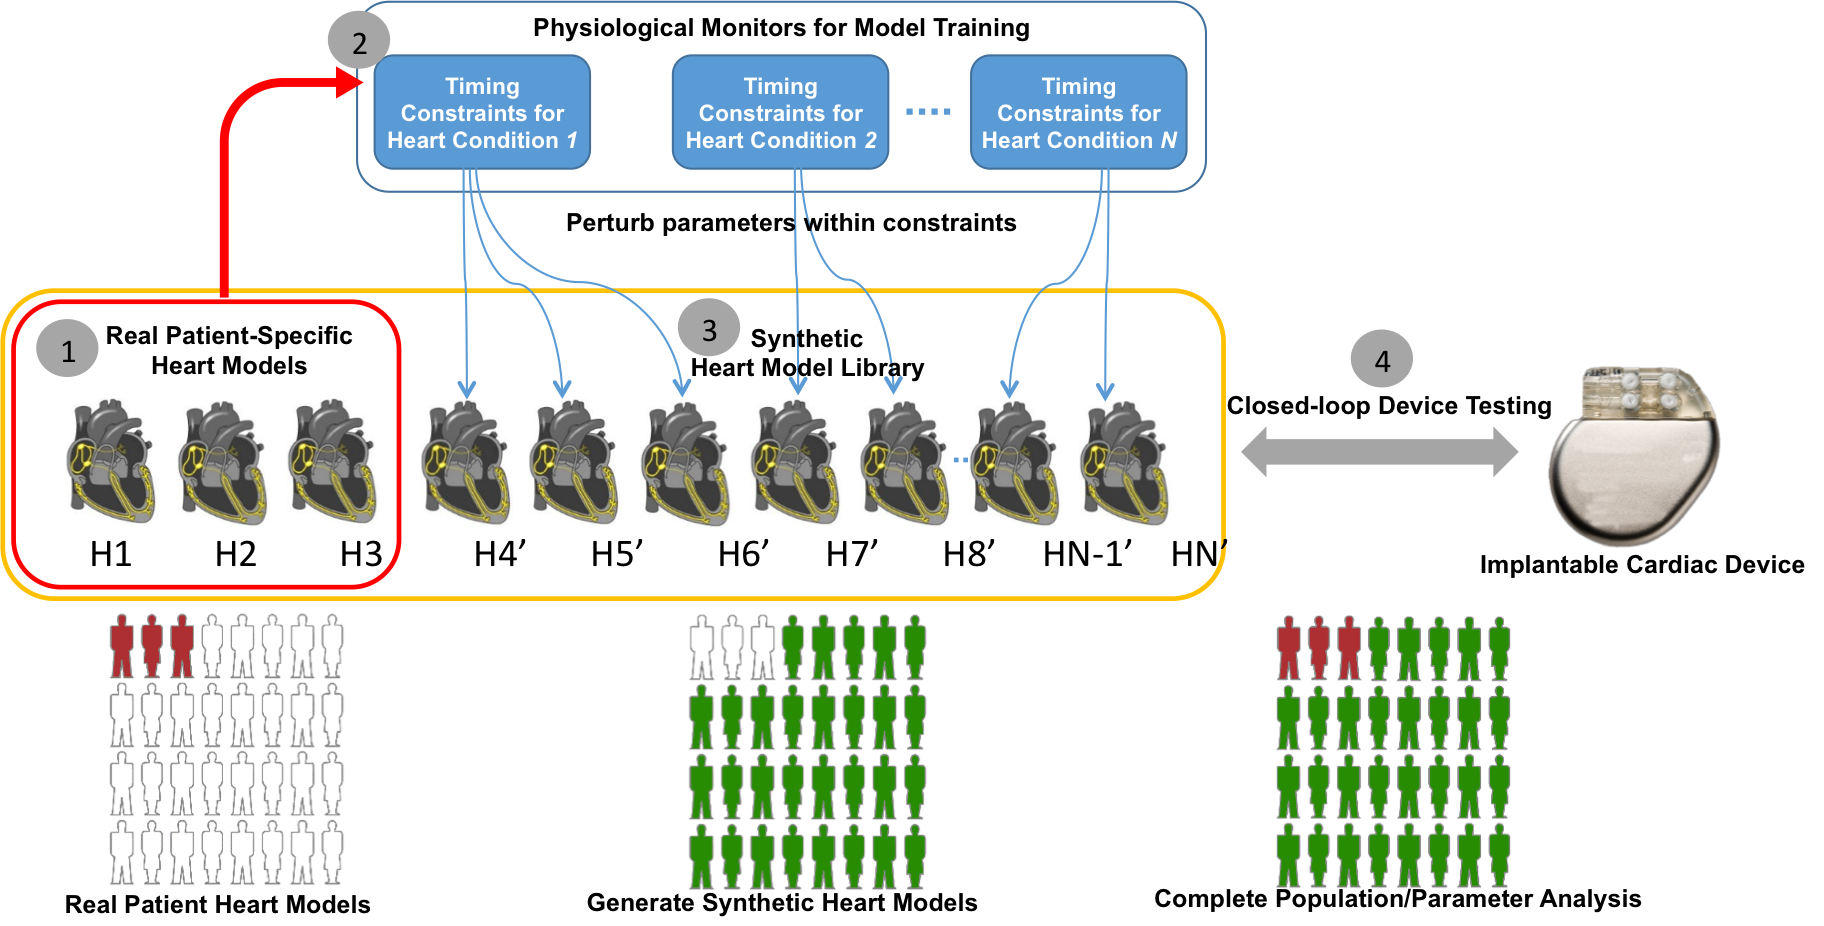
\includegraphics[width=\textwidth]{figs/fig5mbct.png}
	\caption{\small Model-based Clinical Trials}
	\label{fig:mbct}
\end{figure}
(The model cohort is the group of models enrolled in the trial).
Our current approach is to learn the constraints on parameters for the parametrized model using samples of real patients' data, as indicated by markers \circled{1} and \circled{2} in Fig. \ref{fig:mbct}. 
Ideally this sample of patients is a cohort from a previous trial.
These learned constraints are then used to generate more instances of the model (marker \circled{3}), and this constitutes our model cohort.
The device is then connected to these models (marker \circled{4}) and the outcomes of interest are evaluated, such as incidence of adverse events.

%Early efforts tying physiological modeling to clinical trials also include the  which is used to generate simulated patients.

\section{Conclusion}
\yhl{The safety and efficacy of closed-loop medical devices have to be evaluated within their physiological contexts.
In this article we demonstrated how physiological models can be used to provide safety evidence during the development of closed-loop medical devices, which can potentially safe time and cost for the device manufacturers.
Model-based clinical trials have the potential to reduce the scope, cost and probability of failure of clinical trials of medical devices with complex hardware and software. 
MBCT as a rapid certification toolchain to speed up medical device approvals is gaining increasing traction both within the regulatory environment and the medical device industry.
As an example, new diabetes control algorithms can be evaluated on the UVA/PADOVA diabetes model, and the result of which can be used to substitute animal trials \cite{pancreas_paul}. 
These applications can potentially usher a new era of exciting research challenges for the closed-loop verification, validation and testing medical devices at scale. 
}